% ==============================================================================
% SEZIONE 4 — ANALISI CRITICA E CONCLUSIONI
% ==============================================================================
\section[Analisi critica e conclusioni]{Analisi critica e conclusioni: il bilancio energetico reale a livello di sistema}
\label{sec:conclusioni}

I capitoli precedenti hanno messo in evidenza due realtà apparentemente contrapposte: da un lato, singoli neuroni CMOS sottosoglia (come l'Octopus neuron da $<\SI{4}{\pico\joule\per\spike}$ o la piccola rete analogica NET-TEN da appena \SI{3{,}50}{\nano\watt}) dimostrano che il calcolo spiking può raggiungere efficienze energetiche comparabili a quelle dei neuroni biologici; dall'altro, i processori programmabili e i sistemi impiantabili completi consumano da decine di microwatt fino a diversi milliwatt. Diventa dunque essenziale rispondere in modo rigoroso e quantitativo alla domanda critica posta dalla consegna:

\begin{quote}
  \itshape
  «Le SNN offrono un vantaggio energetico concreto per i sistemi biomedicali impiantabili oppure il consumo dei circuiti di acquisizione, delle sinapsi, della memoria e delle interconnessioni può ridimensionare il beneficio ottenuto con neuroni ultra-low-power?»
\end{quote}

L'evidenza sperimentale raccolta nei sette articoli analizzati consente di scomporre il problema lungo quattro assi quantitativi precisi, superando ogni valutazione qualitativa generica.

\subsection{Il paradosso area--energia: il neurone è una frazione minuscola del sistema}
\label{subsec:paradosso_sistema}

\subsubsection{Il peso dominante delle sinapsi (evidenza da ROLLS)}
In una rete neurale, il numero di sinapsi scala molto più rapidamente del numero di neuroni (da decine a migliaia di sinapsi per neurone). Il chip \textbf{ROLLS}~\cite{qiao2015} quantifica questo squilibrio con precisione: nonostante l'accorgimento di condividere un solo circuito DPI per riga tramite la legge di Kirchhoff, i 256 neuroni AdEx-I\&F occupano appena lo \textbf{0,47\%} della superficie del die (\SI{0{,}235}{\milli\meter\squared}), contro il \textbf{64,73\%} (\SI{33{,}28}{\milli\meter\squared}) assorbito dai 128k circuiti sinaptici LTP e STP (Figura~\ref{fig:area_neuroseed}a). Inoltre, i circuiti periferici (BiasGen 2,07\%, interfacce AER 2,59\%, demultiplexer e sinapsi virtuali 1,00\%) superano da soli di oltre dieci volte l'area dei neuroni, e il consumo del sistema in esecuzione sale a circa \SI{4}{\milli\watt}~\cite{qiao2015}. Ridurre ulteriormente l'area o la potenza del singolo soma ha quindi un impatto marginale sul budget complessivo di un processore plastico.

\subsubsection{Il costo della memoria e delle interconnessioni asincrone (evidenza da DYNAPs e DYNAP-SE2)}
Ancora più decisiva è la disaggregazione energetica fornita da Moradi et al.\ (2018)~\cite{moradi2018} per \textbf{DYNAPs} (riportata in Figura~\ref{fig:dynaps_energy}) e ripresa nel modello di potenza di \textbf{DYNAP-SE2} da Bartels et al.\ (2025)~\cite{bartels2025}:
\begin{itemize}
  \item A \textbf{\SI{1{,}8}{\volt}}, generare uno spike nel neurone analogico costa \SI{883}{\pico\joule} (e l'estensore di impulso \SI{324}{\pico\joule}), ma la codifica dell'indirizzo richiede altri \SI{883}{\pico\joule}, il routing verso un altro core \SI{360}{\pico\joule} e il solo \textbf{broadcast nella memoria associativa CAM locale} divora \textbf{\SI{6{,}84}{\nano\joule}} (\SI{6840}{\pico\joule}) — cioè \textbf{7,7 volte} l'energia di generazione dello spike! Su un totale di \SI{9{,}29}{\nano\joule} per un evento instradato tra core diversi, oltre il \textbf{73,6\%} è speso nel solo broadcast CAM e l'\textbf{87,0\%} complessivo va in memoria, codifica e interconnessioni digitali, mentre il neurone pesa per appena il \textbf{9,5\%}.
  \item Riducendo la tensione a \textbf{\SI{1{,}3}{\volt}}, lo squilibrio si accentua ulteriormente: generare uno spike scende a \SI{260}{\pico\joule}, ma il broadcast CAM costa \textbf{\SI{2{,}20}{\nano\joule}} (\textbf{8,5 volte} la generazione dello spike), portando l'infrastruttura di comunicazione e memoria a superare il \textbf{90\%} dell'energia per evento!
  \item Anche in termini di silicio, memoria on-chip (31,7\%), pulse extender/decoder (25,2\%) e router (9,7\%) coprono il \textbf{66,6\%} dell'area core di DYNAPs, contro il 22,8\% di neuroni e sinapsi~\cite{moradi2018}.
\end{itemize}

% --- FIGURA 4.1: Disaggregazione energetica DYNAPs (Moradi 2018 Tab. III) ---
\begin{figure}[tb]
  \centering
  \begin{tikzpicture}
    \begin{axis}[
      ybar,
      bar width=14pt,
      width=0.92\textwidth,
      height=5.7cm,
      ylabel={Energia per evento (\si{\pico\joule})},
      symbolic x coords={Gen.\ spike, Est.\ impulso, Codifica+SRAM, Routing core, Broadcast CAM},
      xtick=data,
      ymin=0, ymax=7900,
      ymajorgrids=true,
      grid style={dashed, color=RuleGray},
      nodes near coords,
      nodes near coords align={vertical},
      every node near coord/.append style={font=\tiny\bfseries, /pgf/number format/1000 sep={\,}},
      yticklabel style={/pgf/number format/1000 sep={\,}},
      legend style={at={(0.03,0.94)}, anchor=north west, font=\scriptsize, draw=RuleGray},
      tick label style={font=\scriptsize},
      label style={font=\footnotesize},
      enlarge x limits=0.14
    ]
      \addplot[fill=black!78, draw=black] coordinates {
        (Gen.\ spike, 883)
        (Est.\ impulso, 324)
        (Codifica+SRAM, 883)
        (Routing core, 360)
        (Broadcast CAM, 6840)
      };
      \addplot[fill=black!28, draw=black] coordinates {
        (Gen.\ spike, 260)
        (Est.\ impulso, 26)
        (Codifica+SRAM, 507)
        (Routing core, 78)
        (Broadcast CAM, 2200)
      };
      \legend{$\Vdd = \SI{1{,}8}{\volt}$ (tot.\ \SI{9{,}29}{\nano\joule}), $\Vdd = \SI{1{,}3}{\volt}$ (tot.\ \SI{3{,}07}{\nano\joule})}
    \end{axis}
  \end{tikzpicture}
  \caption[Disaggregazione dell'energia per evento in DYNAPs]{Disaggregazione quantitativa dell'energia per singola operazione nel processore DYNAPs a \SI{1{,}8}{\volt} e \SI{1{,}3}{\volt} (dati sperimentali da Moradi et al., 2018, Tabella~III~\cite{moradi2018}). Il solo broadcast nella CAM del core supera di $7{,}7\text{--}8{,}5\times$ l'energia richiesta dal neurone analogico per generare lo spike.}
  \label{fig:dynaps_energy}
\end{figure}

\subsubsection{Il limite fisico del front-end di acquisizione (NET-TEN vs NeuroSEED e Xylo)}
Il terzo elemento decisivo emerge confrontando un core SNN isolato come \textbf{NET-TEN} (\SI{3{,}50}{\nano\watt})~\cite{ronchini2023} con un SoC impiantabile completo come \textbf{NeuroSEED} (\SI{63{,}61}{\micro\watt})~\cite{wu2026}. NET-TEN raggiunge consumi nell'ordine dei nanowatt perché esclude del tutto l'acquisizione amplificata del segnale microvoltico dagli elettrodi, la cancellazione dell'offset DC elettrochimico, la conversione analogico-spike (svolta in MATLAB) e la stimolazione/telemetria. Quando invece si costruisce un sistema reale che deve acquisire segnali neurali dell'ordine delle decine di microvolt con un rumore riferito all'ingresso accettabile (IRN $= \SI{2{,}9}{\micro\volt\textsubscript{rms}}$ in NeuroSEED), si incontra un \textbf{limite fisico fondamentale imposto dal rumore termico} sulla banda di acquisizione: per contenere il rumore integrato occorre mantenere un'adeguata transconduttanza $g_m$ — e quindi una corrente statica di polarizzazione dell'LNA, ottimizzabile tramite inversione debole ($g_m/I_D \approx 26$) e basso \emph{Noise Efficiency Factor} (NEF) — non comprimibile arbitrariamente~\cite{wu2026}.

Come mostra inequivocabilmente la Figura~\ref{fig:area_neuroseed}b, nel SoC completo NeuroSEED il solo \textbf{front-end analogico di acquisizione (AFE)} assorbe \textbf{\SI{38{,}4}{\micro\watt}}, pari al \textbf{60,4\%} dell'intera potenza del chip (seguito dal rivelatore di spike con il 24,2\%, dall'ASC con l'8,2\% e dal trasmettitore IR-UWB con il 7,2\%)~\cite{wu2026}. Anche nei sistemi di rilevamento epilettico su EEG di scalpo come \textbf{Xylo}~\cite{li2024}, i \SI{287{,}9}{\micro\watt} del core SNN digitale rappresentano solo una frazione del budget di un dispositivo reale, poiché vanno aggiunti \SI{87{,}4}{\micro\watt} di I/O SPI, l'AFE multicanale e il pre-filtraggio/rimozione artefatti (che in~\cite{li2024} include ICA off-chip, operazione molto onerosa se portata on-chip).

% --- FIGURA 4.2: Area breakdown comparativa + Pie charts NeuroSEED ---
\begin{figure}[tb]
  \centering
  \begin{subfigure}[b]{0.50\textwidth}
    \centering
    \resizebox{\linewidth}{!}{%
    \begin{tikzpicture}
      \begin{axis}[
        xbar stacked,
        bar width=16pt,
        width=7.4cm,
        height=4.8cm,
        xlabel={Quota di area di silicio (\%)},
        symbolic y coords={NeuroSEED, DYNAPs, ROLLS},
        ytick=data,
        xmin=0, xmax=100,
        tick label style={font=\scriptsize},
        label style={font=\footnotesize},
        legend style={at={(0.46,1.04)}, anchor=south, legend columns=2, font=\tiny, draw=RuleGray},
        nodes near coords,
        nodes near coords style={font=\tiny, color=white, /pgf/number format/fixed, /pgf/number format/precision=1, /pgf/number format/use comma},
        visualization depends on={rawx \as \myx},
        every node near coord/.append style={
          /pgfplots/check for zero/.code={
            \ifdim\myx pt<5pt
              \pgfkeysalso{opacity=0}
            \fi
          },
          /pgfplots/check for zero
        }
      ]
        % 1. Neuroni / Detector (core computazionale puro)
        \addplot[fill=black!85, draw=white] coordinates {(0.5,ROLLS) (22.8,DYNAPs) (15.0,NeuroSEED)};
        % 2. Sinapsi / Memoria (LTP+STP in ROLLS; Memoria+PE/DEC in DYNAPs; ASC in NeuroSEED)
        \addplot[fill=black!60, draw=white] coordinates {(65.3,ROLLS) (56.9,DYNAPs) (31.3,NeuroSEED)};
        % 3. Routing / I/O / UWB TX
        \addplot[fill=black!40, draw=white] coordinates {(3.0,ROLLS) (9.7,DYNAPs) (21.2,NeuroSEED)};
        % 4. AFE / BiasGen / Pad & Altro
        \addplot[fill=black!20, draw=black!50, every node near coord/.append style={color=black}] coordinates {(31.2,ROLLS) (10.6,DYNAPs) (32.5,NeuroSEED)};
        \legend{Neuroni / Det.\ (n+s DYN.), Sinapsi / Mem.+PE / ASC, Routing / AER / UWB, AFE / BiasGen / Altro}
      \end{axis}
    \end{tikzpicture}%
    }
    \caption{Ripartizione dell'area in ROLLS (neur.\ 0,5\%), DYNAPs e NeuroSEED.}
  \end{subfigure}
  \hfill
  \begin{subfigure}[b]{0.47\textwidth}
    \centering
    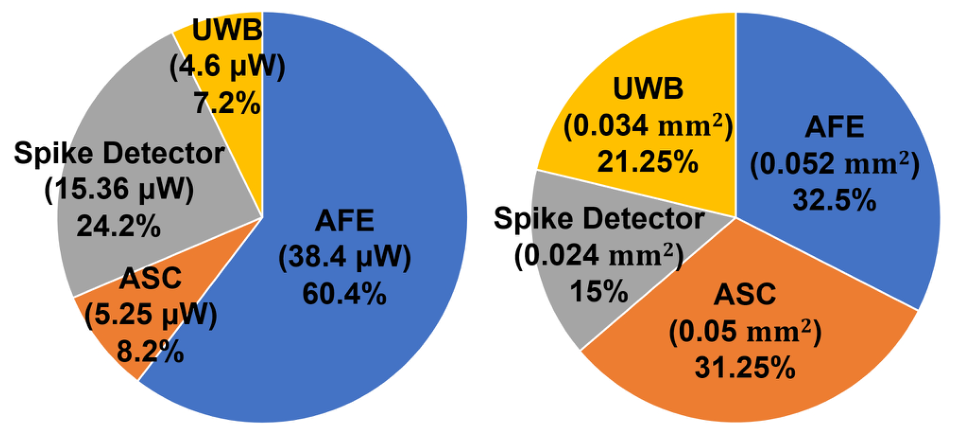
\includegraphics[width=\linewidth]{neuroseed_breakdown.png}
    \caption{Potenza (\SI{63{,}61}{\micro\watt}) e area attiva (\SI{0{,}16}{\milli\meter\squared}) in NeuroSEED~\cite{wu2026}.}
  \end{subfigure}
  \caption[Ripartizione di area e potenza: il peso dell'infrastruttura]{Evidenza quantitativa del peso dell'infrastruttura rispetto al core di calcolo: (a) distribuzione percentuale dell'area di silicio in ROLLS~\cite{qiao2015} (neuroni 0,47\% vs sinapsi 64,73\%, pad/altro $\sim 31\%$), DYNAPs~\cite{moradi2018} (core: memoria+PE/DEC 56,9\%, router 9,7\%, neuroni+sinapsi 22,8\%) e NeuroSEED~\cite{wu2026} (area attiva); (b) grafici a torta originali di potenza e area di NeuroSEED~\cite{wu2026}, in cui il front-end analogico AFE domina con il 60,4\% della potenza totale.}
  \label{fig:area_neuroseed}
\end{figure}

% --- FIGURA 4.3: Confronto logaritmico potenze di sistema ---
\begin{figure}[tb]
  \centering
  \resizebox{\textwidth}{!}{%
  \begin{tikzpicture}
    \begin{axis}[
      xbar,
      xmode=log,
      log origin=infty,
      bar width=11pt,
      width=12.4cm,
      height=5.9cm,
      xlabel={Potenza media di sistema in scala logaritmica (\si{\micro\watt})},
      ytick={1,2,3,4,5,6,7},
      yticklabels={
        {FPGA conv.\ (SVM/MLP)},
        {ROLLS (128k sin.\ plast.)},
        {Sharifshazileh (SNN+AFE)},
        {Xylo (SNN dig.\ + I/O)},
        {DYNAP-SE2 (iEEG 42--62ch)},
        {NeuroSEED (32ch AFE+TX)},
        {NET-TEN (solo core SNN)}
      },
      ymin=0.4, ymax=7.6,
      xmin=0.001, xmax=35000000,
      xmajorgrids=true,
      grid style={dashed, color=RuleGray},
      tick label style={font=\scriptsize},
      label style={font=\footnotesize},
      nodes near coords,
      point meta=explicit symbolic,
      every node near coord/.append style={font=\tiny\bfseries, anchor=west, xshift=3pt}
    ]
      \addplot[fill=black!55, draw=black] coordinates {
        (0.0035, 7) [\SI{3{,}50}{\nano\watt} (senza AFE/TX)]
        (63.61, 6) [\SI{63{,}61}{\micro\watt} (SoC completo)]
        (150, 5) [\SI{150}{\micro\watt} (\SI{2{,}8}{\micro\watt\per\ch})]
        (375.3, 4) [\SI{375{,}3}{\micro\watt} (senza AFE/ICA)]
        (555.6, 3) [\SI{555{,}6}{\micro\watt} (con AFE)]
        (4000, 2) [\SI{4}{\milli\watt} (apprend.\ on-line)]
        (220000, 1) [$160\text{--}\SI{284}{\milli\watt}$]
      };
    \end{axis}
  \end{tikzpicture}%
  }
  \caption[Confronto logaritmico delle potenze di sistema]{Confronto su scala logaritmica (nove ordini di grandezza) della potenza media dei sistemi analizzati: il passaggio dal solo nucleo SNN analogico (NET-TEN, \SI{3{,}5}{\nano\watt}) a un SoC impiantabile completo con acquisizione AFE e telemetria (NeuroSEED, \SI{63{,}6}{\micro\watt}) o a un processore SNN riconfigurabile (DYNAP-SE2, Xylo, ROLLS) ridimensiona drasticamente il guadagno del singolo neurone, pur conservando un margine decisivo ($10^2\text{--}10^3\times$) rispetto alle architetture digitali convenzionali su FPGA.}
  \label{fig:power_landscape}
\end{figure}

\FloatBarrier
\subsection{Sintesi dei colli di bottiglia e strategie di mitigazione}
\label{subsec:colli_bottiglia}

La Tabella~\ref{tab:colli_bottiglia} raccoglie in forma sintetica i quattro principali colli di bottiglia emersi dalla letteratura e le rispettive vie di soluzione architetturali e tecnologiche.

\begin{table}[htb]
  \centering
  \vspace{-4pt}
  \caption[Colli di bottiglia energetici e strategie di mitigazione]{Sintesi critica dei colli di bottiglia energetici e di area nei sistemi impiantabili basati su SNN e relative strategie di mitigazione emerse dalla bibliografia.}
  \label{tab:colli_bottiglia}
  \scriptsize
  \renewcommand{\arraystretch}{0.98}
  \setlength{\tabcolsep}{4pt}
  \begin{tabularx}{\textwidth}{@{}L{2.3cm} L{3.25cm} Y Y@{}}
    \toprule
    \textbf{Blocco critico} & \textbf{Evidenza quantitativa} & \textbf{Origine fisica / architetturale} & \textbf{Strategie di mitigazione} \\
    \midrule
    \textbf{Front-end di acquisizione (AFE)} & NeuroSEED: \SI{38{,}4}{\micro\watt} (\textbf{60,4\%} della potenza del SoC; 32,5\% area)~\cite{wu2026}. & Limite del rumore termico in banda (compromesso $g_m/I_D$ e NEF) e cancellazione offset DC elettrodico ($\pm\SI{50}{\milli\volt}$). & Multiplexing diretto TDM + LNA \emph{current-reuse} in sottosoglia (NEF 2,1) + servo-loop digitale EDO + codifica ADM/ASC integrata~\cite{wu2026, bartels2025}. \\
    \textbf{Sinapsi e memoria pesi} & ROLLS: \textbf{64,73\%} area per sinapsi vs 0,47\% neuroni~\cite{qiao2015}; NET-TEN: ritenzione $C_w$ solo decine di ms~\cite{ronchini2023}. & Fan-in/fan-out elevato; perdita di carica sui condensatori analogici; costo delle celle SRAM/bistabili. & Condivisione DPI per riga~\cite{qiao2015}; topologie sparse e pesi quantizzati/costanti~\cite{ronchini2023, bartels2025}; memorie non volatili emergenti (ReRAM / memristori)~\cite{moradi2018, indiveri2011}. \\
    \textbf{Interconnessioni e routing (CAM/AER)} & DYNAPs: broadcast CAM \textbf{\SI{6{,}84}{\nano\joule}} (\SI{1{,}8}{\volt}) / \textbf{\SI{2{,}2}{\nano\joule}} (\SI{1{,}3}{\volt}), ovvero $7{,}7\text{--}8{,}5\times$ la gen.\ dello spike~\cite{moradi2018}. & Carica/scarica delle linee di ricerca e \emph{match-line} su grandi array di CAM e bus digitali. & Routing gerarchico a due stadi basato su tag (Eq.~\ref{eq:dynaps_mem}); scalatura a nodi avanzati (\SI{28}{\nano\meter} FDSOI)~\cite{moradi2018}; reti dedicate senza bus AER dove non serve riconfigurabilità~\cite{ronchini2023}. \\
    \textbf{Variabilità (\emph{mismatch}) e post-processing} & DYNAP-SE2: CV bias 20--30\%~\cite{bartels2025}; NET-TEN: 4/10 canali utili; Xylo: $-3{,}5\text{--}4{,}3\%$ acc.\ da quant.\ 8 bit~\cite{li2024}. & Dispersione esponenziale di $I_D$ in sottosoglia ($\Delta V_{\mathrm{th}}$) e sensibilità alla densità di codifica. & Sovradimensionamento mirato (ROLLS: 9,4\%~\cite{qiao2015}); reti a popolazione/topologia robusta (NLNG~\cite{bartels2025}); apprendimento omeostatico on-chip; contatori ultra-low-power on-chip~\cite{ronchini2023}. \\
    \bottomrule
  \end{tabularx}
  \vspace{-6pt}
\end{table}

\FloatBarrier
\vspace{-4pt}
\subsection{Verdetto conclusivo}
\label{subsec:verdetto}

\begin{criticaBox}[top=5pt, bottom=5pt, before skip=2pt, after skip=2pt]{Conclusione critica: le SNN offrono davvero un vantaggio energetico concreto negli impianti biomedicali?}
{\footnotesize\setlength{\baselineskip}{10.5pt}
L'analisi comparativa integrata conduce a una risposta netta e articolata in due parti complementari:
\begin{enumerate}[topsep=2pt, itemsep=1.5pt]
  \item \textbf{Sì, il consumo dell'infrastruttura ridimensiona drasticamente il beneficio isolato del singolo neurone ultra-low-power.} Parlare di ``processori da pochi nanowatt'' guardando solo il core analogico (come i \SI{3{,}50}{\nano\watt} di NET-TEN) è fuorviante se non si include il costo del resto della catena: in un dispositivo impiantabile reale, il front-end analogico di acquisizione (60,4\% della potenza in NeuroSEED), le sinapsi (64,7\% dell'area in ROLLS) e soprattutto la memoria associativa e le interconnessioni di routing (fino all'87--90\% dell'energia per evento in DYNAPs) dominano di \textbf{uno fino a quattro ordini di grandezza} rispetto al consumo intrinseco del soma neuronale (Figura~\ref{fig:power_landscape}).
  \item \textbf{Ciononostante, il paradigma SNN/\emph{event-driven} offre un vantaggio energetico e sistemistico concreto e decisivo, a patto che sia co-progettato a livello di intero sistema.} Il vero guadagno delle SNN impiantabili non deriva tanto dal risparmiare qualche picojoule nel singolo neurone, bensì dal loro impatto a cascata sull'intera architettura del dispositivo:
  \begin{itemize}[topsep=1.5pt, itemsep=1pt]
    \item \textbf{Abbattimento della telemetria wireless:} elaborare ed estrarre eventi localmente comprime il flusso dati di oltre $500\times$ (NeuroSEED riduce il trasmettitore IR-UWB a soli \SI{4{,}6}{\micro\watt}, appena il 7,2\% del chip), risolvendo il collo di bottiglia energetico più critico delle interfacce multicanale ad alta densità.
    \item \textbf{Eliminazione di buffer, ADC Nyquist continui e clock globali:} l'elaborazione asincrona in \emph{streaming} consente latenze di decine di millisecondi (essenziali per la neuromodulazione \emph{closed-loop} dell'epilessia) e un consumo strettamente modulato dall'occorrenza di eventi patologici, con un guadagno di $10^2\text{--}10^3\times$ rispetto a implementazioni convenzionali su FPGA o microprocessori general-purpose.
  \end{itemize}
\end{enumerate}
In prospettiva, la maturità clinica dei sistemi biomedicali impiantabili neuromorfici non dipenderà quindi dall'ulteriore miniaturizzazione isolata del neurone LIF/AdEx, bensì dalla \textbf{co-progettazione olistica \emph{end-to-end}} di front-end compatti a basso rumore (TDM/ADM/ASC), topologie SNN sparse intrinsecamente robuste al \emph{mismatch} (o capaci di adattamento omeostatico locale), stadi di decisione/classificazione interamente on-chip e tecnologie di memoria non volatile integrata (come ReRAM) capaci di abbattere il costo energetico di sinapsi e routing.
}
\end{criticaBox}
